  
  In this chapter the results for the US Airline Passenger Dataset are
  presented. First, the model specifications and results of graph
  representation learning and GNNs are presented. Afterwards, the graph machine
  learning results are compared to the results using "standard" machine
  learning methods.

  \section{Graph Representation Learning}

  The graph generated in section \ref{section:graph_gen} using the MAG method
  was used for graph representation learning. The Node2Vec algorithm using an
  unbiased walk was employed for learning the 2-dimensional node representations 
  of the graph. The Node2Vec algorithm was employed using following model 
  parameters:

  \begin{itemize}
    \setlength\itemsep{0.1em}
    \item Embedding size $d$: 2
    \item Random walk length $t$: 8
    \item Number of random walks $\gamma$: 100
    \item Window size $w$: 10
    \item Node batch size: 2
    \item Return parameter $p=1$
    \item In-out parameter $q=1$
  \end{itemize}

  \noindent With the specified return- and in-out parameters, the Node2Vec
  output corresponds to the DeepWalk output. The resulting node embeddings were
  then used as inputs for standard machine learning methods. The resulting node 
  embeddings are shown in figure \ref{fig:node2vec}. 

  \begin{figure}[h]
		\centering
		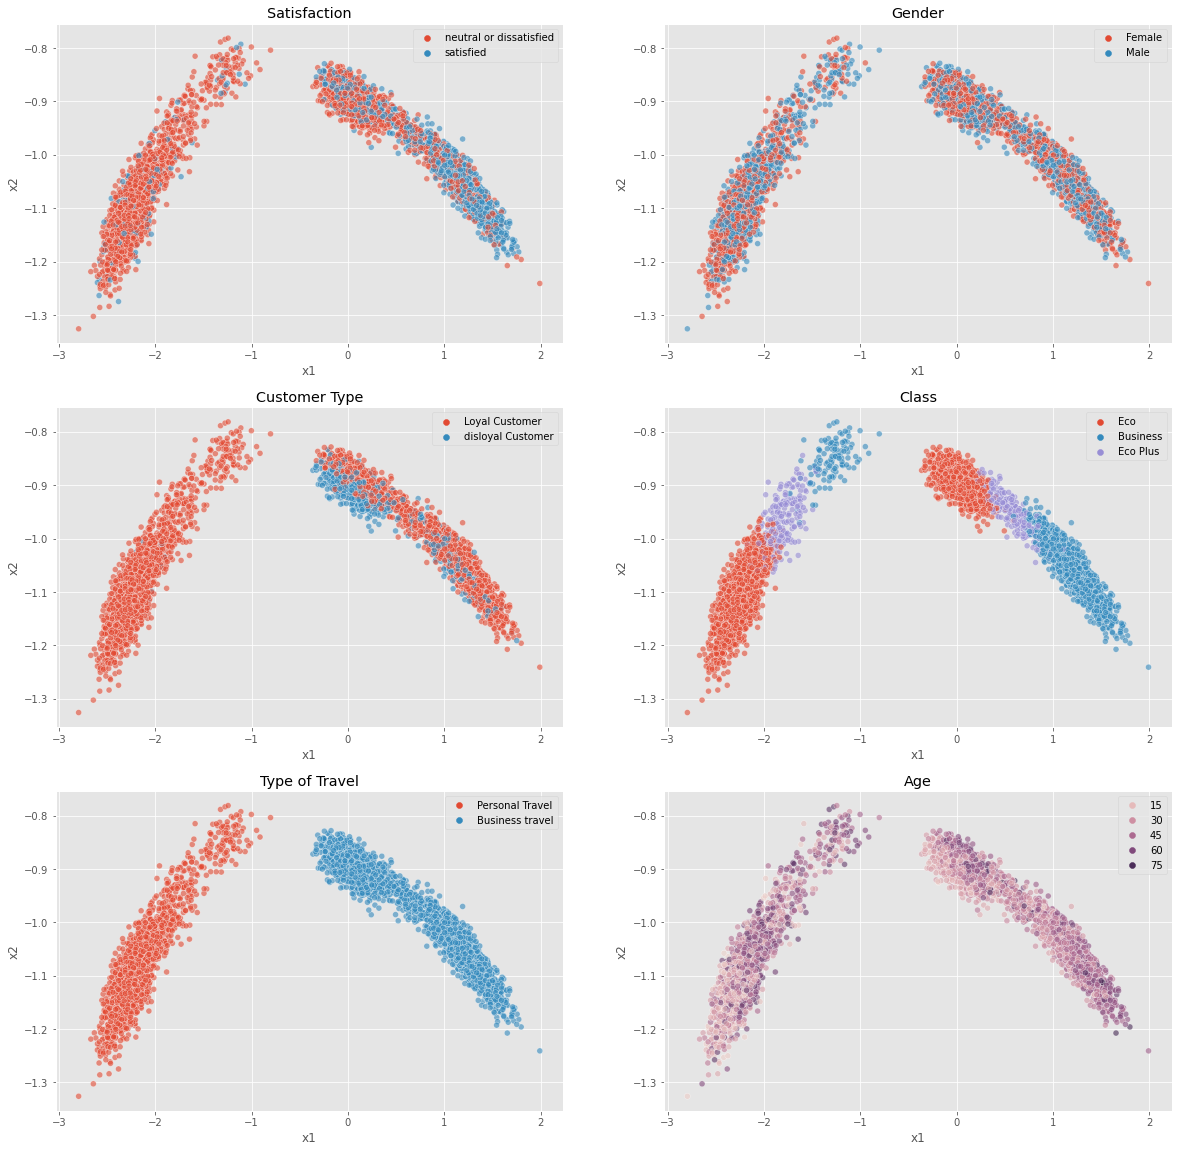
\includegraphics[width=0.9\textwidth]{node2vec_emb.png}
		\caption{Node2Vec embeddings}
        \label{fig:node2vec}
  \end{figure}

  \noindent The plotted node embeddings in figure \ref{fig:node2vec} reveal 
  interesting neighborhood structures. First, the nodes are split according to
  their type of travel. This corresponds to the two main clusters shown in
  figure \ref{fig:us_airline_graph}. Secondly, the node embeddings are grouped 
  in a nice and orderly fashion. The node embeddings are part of Euclidean
  space, which is why the plots shown in figure \ref{fig:node2vec} are proper
  scatter plots. This allows for direct comparison of nodes and the groups
  which they belong to. The 2-dimensional node embeddings thus provide 
  interesting insights via data visualization.\\

  \noindent The node embeddings were used as input data for the three standard 
  machine learning methods shown in table \ref{table:node2vec_results}.

  \begin{table}[h]
    \centering
    \begin{tabular}{|l||l|l|}
      \hline
      \textbf{ML Method} & \textbf{Training Accuracy} & \textbf{Validation
      Accuracy}\\
      \hline\hline
      Logistic Regression & 76.85\% & 75.83\% \\\hline 
      Support Vector Machine & 76.95\% & 75.66\% \\\hline
      ANN & 77.61\% & 76.58\% \\
      \hline
    \end{tabular}
    \caption{Node2Vec Classification Results}
    \label{table:node2vec_results}
  \end{table}

  \noindent The results show, that Node2Vec only has very modest success in
  classifying passengers according to their satisfaction. Applying the trained
  models to the test data yielded even more inferior results. When looking at the
  satisfaction scatter plot in figure \ref{fig:node2vec}, it becomes obvious why
  the downstream machine learning tasks only had limited success. The
  attributes used for generating the graph, for which neighborhood
  clusters emerged, Node2Vec created very good node embeddings. The label 
  satisfaction could not be used as an attribute for graph generation as this 
  would be unrealistic. As the label is not considered for graph generation,
  Node2Vec does not create embeddings which directly consider the label. The 
  label is only considered to the extend that the attributes create structures 
  which are related with the label. For that reason, the success of any 
  downstream machine learning method will be limited to the extent that the node 
  embeddings capture relevant information for predicting the label. \\

  \noindent Alternative model specifications were tested, which mainly included
  learning higher dimensional node embeddings. These node embeddings however
  did not yield better results. Given the almost identical accuracies, the more
  parsimonious model with 2 dimensions is preferred. As a final test, the node
  embeddings were joined to the feature data presented in section 
  \ref{section:airline_data}. This data was then used as the input data for the
  downstream machine learning models. For the training- and validation data,
  this approach yielded excellent results with accuracies $\approx 95\%$. 
  Unfortunately, this did not translate to the test data, which resulted in an 
  accuracy of approximately 89\%. In addition, the results presented in section
  \ref{section:result_comp} show, that similar accuracies are achieved
  only using the feature data. The trained model excluding the node embeddings
  also performs well for test data. For that reason, joining feature data with 
  node embeddings is not a recommended approach for the US Airline Passenger
  dataset.

  \section{Graph Neural Networks}

  This section presents the results using graph neural networks. As
  mentioned in section \ref{section:GNN_theory}, GCN by \cite{kipf2016semi} and
  GraphSage by \cite{hamilton2017inductive} are used for classifying the
  satisfaction of the US airline passengers. The model specifications 
  and results are presented in the following sections for both methods.

  \subsection{Graph Convolutional Network}

  The GCN was designed using the forward propagation function already shown in 
  equation \ref{eq:GCN_forward}.

  \begin{equation}
	  Z = f(X,A) = \text{softmax}\left(\hat A \;\text{ReLu}\left(\hat A X
	  W^{(0)}\right)W^{(1)}\right)
      \label{eq:GCN_forward_1}
  \end{equation}

  \noindent The node features $X$ include to the 21 explanatory variables of the 
  US airline passenger dataset as described in section 
  \ref{section:airline_data}. The categorical variables were dummy coded, which
  is why the feature matrix includes 24 variables. The hidden layer size of the 
  convolutional layers was set to 128 and the output layer was set to size 
  2 for the binary classification task. The training loss was calculated using 
  cross-entropy loss and the model parameters were updated using the Adam 
  optimizer \citep{kingma2014adam} with the learning rate set to $0.002$. 
  Essentially, algorithm \ref{algo:GNN_struct} ca be applied by replacing the 
  forward propagation with equation \ref{eq:GCN_forward_1} and updating the 
  model parameters using the Adam optimizer instead of standard gradient descent.
  Different model specification were tested, however the chosen specifications
  appeared to perform best. The GCN required approximately 1'200 epochs to 
  finish training. This large number of epochs is due to the full-batch
  training procedure employed for the GCN. Mini-batch training can
  unfortunately not be applied for GCNs. The resulting loss- and accuracy plots 
  are shown in figure \ref{fig:gcn_plots}.

  \begin{figure}[h]
		\centering
		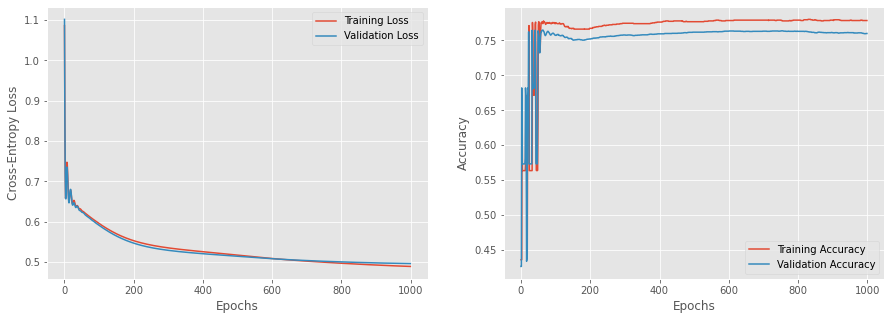
\includegraphics[width=0.9\textwidth]{gcn_plots.png}
		\caption{GCN Loss- and Accuracy Plots}
        \label{fig:gcn_plots}
  \end{figure}

  \noindent The resulting confusion matrices and the final accuracies are 
  further presented in tables \ref{table:gcn_results_train} \& 
  \ref{table:gcn_results_valid}. 

  \begin{table}[h]
    \centering
    \begin{tabular}{|l|c|c|}
      \hline
      \diagbox{\textbf{Label}}{\textbf{Predicted}} & \textbf{Neutral or
      Dissatisfied} & \textbf{Satisfied}\\
      \hline
      \textbf{Neutral or Dissatisfied} & 893 & 143 \\\hline 
      \textbf{Satisfied} & 148 & 605 \\\hline\hline
      \textbf{Accuracy} & 83.73\% & \\
      \hline
    \end{tabular}
    \caption{Confusion Matrix Training Data}
    \label{table:gcn_results_train}
  \end{table}

  \begin{table}[h]
    \centering
    \begin{tabular}{|l|c|c|}
      \hline
      \diagbox{\textbf{Label}}{\textbf{Predicted}} & \textbf{Neutral or
      Dissatisfied} & \textbf{Satisfied}\\
      \hline
      \textbf{Neutral or Dissatisfied} & 2'004 & 383 \\\hline 
      \textbf{Satisfied} & 339 & 1'485 \\\hline\hline
      \textbf{Accuracy} & 82.85\% & \\
      \hline
    \end{tabular}
    \caption{Confusion Matrix Validation Data}
    \label{table:gcn_results_valid}
  \end{table}

  \noindent Graph convolutional networks are designed to be used in a
  transductive setting and the model cannot be applied to new and unseen
  graphs. In this setting 30\% of the dataset was used for training and 70\% of
  the data was used for validation. This is done by masking the nodes in the
  graph which are part of the validations dataset. The masked nodes are 
  considered in the in the neighborhood function $\mathcal{N}(v)$, they are 
  however not considered as target nodes. Therefore, masked nodes are not use
  for updating the model parameters. The fact, that GCNs cannot be used in an
  inductive setting is very limiting. Further, the GCN requires over 1'200
  epochs to start finish training and yields only mediocre results in terms of
  accuracy and model fit. A reason for this could be that only a full-batch
  implementation for GCN was introduced. In addition, GCNs always consider the
  entire neighborhood set. Sampling the neighborhood and mini-batch training 
  which is an important ingredient of GraphSage and is introduced as an
  improved and superior GNN method in the following subsection.

  \subsection{GraphSage}

  For GraphSage the exact same data input was used as for the GCN. The 
  GraphSage model included 2 convolutional layers where both have a hidden 
  layer size of 128 and the output layer is of size 2. The model is defined
  using an adaptation of algorithm \ref{algo:GraphSage}. Similar as for the 
  GCN, the training graph is split into 80\% training and 20\% validation using 
  node masking. The loss is calculated using cross-entropy and the model 
  parameters are updated using the Adam optimizer with the learning rate set to 
  0.002 and is an adaptation to the model updating procedure shown in 
  algorithm \ref{algo:GNN_struct}. The output of the first convolutional layer 
  is activated using the ReLu function and the output of the second 
  convolutional layer is activated using the log-softmax function. The model was 
  trained using a mini-batch size of 50 nodes and the neighborhood function 
  $\mathcal{N}(v)$ randomly sampled 10 neighbors 2-hops away from the target
  node and randomly sampled 5 nodes at a 1-hop distance from the target node. 
  This corresponds to the steps shown in figure \ref{fig:GraphSage_sample}. 
  To improve the robustness of the model, lastly a dropout rate of $p = 0.02$ 
  was set. GraphSage was run using the different aggregation strategies mean, 
  LSTM, max-pooling. In addition, sum-pooling was added as an additional 
  aggregation strategy as suggested by \cite{xu2018powerful}. Sum-pooling 
  aggregation follows the same procedure as max-pooling with the only difference 
  being that element-wise sum-pooling is performed and not max-pooling. This 
  aggregation method has been shown to be more robust for graph neural networks, 
  as it allows the GNN to better distinguish different graph structures. It is
  important to note, that the Graphsage sum-pooling strategy employed does not
  correspond to the Graph Isomorphism Network introduced by 
  \cite{xu2018powerful}. This article rather provided the inspiration for
  applying sum-pooling for Graphsage. \\
  
  \noindent The model for each aggregation strategy was trained using 400 epochs. 
  The training- and validation results using the training graph are presented 
  for every aggregation strategy. In addition, the trained models are applied 
  to a new unseen graph also consisting of 6'000 nodes to check for the 
  inductive capability of the Graphsage model. 

  \paragraph{Mean Aggregation}  \mbox{}\\ 
  In figure \ref{fig:mean_aggregation} the training- and validation loss as
  well as the accuracies for the mean aggregation model is shown.

  \begin{figure}[h]
		\centering
		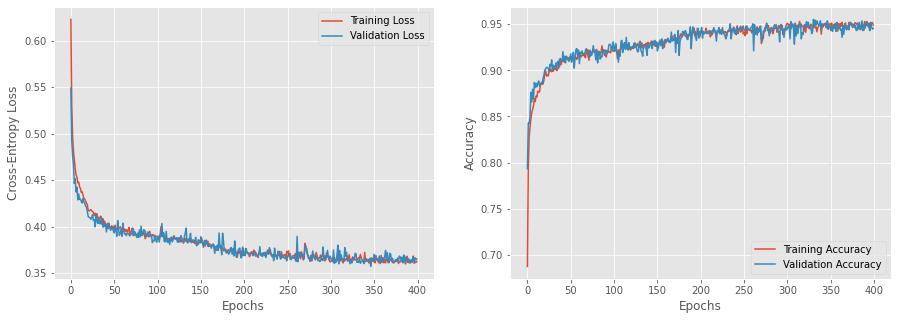
\includegraphics[width=0.9\textwidth]{graphsage_mean_plots.png}
		\caption{Mean Aggregation Loss- and Accuracy Plots}
        \label{fig:mean_aggregation}
  \end{figure}

  \noindent The training accuracy is 94.98\% and the validation accuracy is 
  94.59\% after 400 epochs. The model resulted in a test accuracy of 93.38\%
  with the following confusion matrix shown in table
  \ref{table:mean_results_test}:


  \begin{table}[h]
    \centering
    \begin{tabular}{|l|c|c|}
      \hline
      \diagbox{\textbf{Label}}{\textbf{Predicted}} & \textbf{Neutral or
      Dissatisfied} & \textbf{Satisfied}\\
      \hline
      \textbf{Neutral or Dissatisfied} & 3'262  & 94 \\\hline 
      \textbf{Satisfied} & 303 & 2'341 \\\hline\hline
      \textbf{Accuracy} & 93.38\% & \\
      \hline
    \end{tabular}
    \caption{Test Confusion Matrix Mean Aggregation}
    \label{table:mean_results_test}
  \end{table}

  \paragraph{LSTM Aggregation}  \mbox{}\\ 
  Figure \ref{fig:lstm_aggregation} shows the training- and validation loss
  and accuracy using LSTM aggregation. 

  \begin{figure}[h]
		\centering
		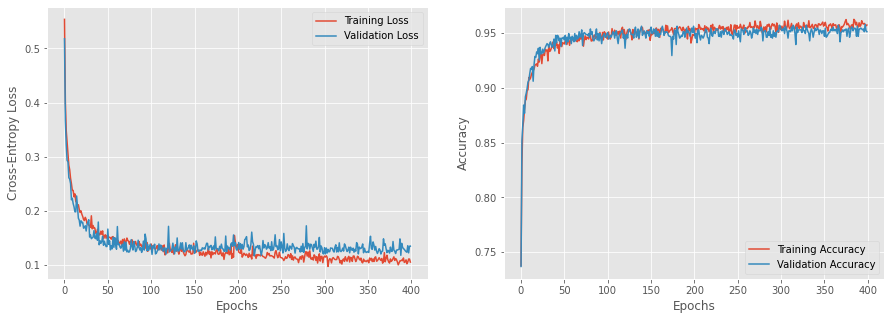
\includegraphics[width=0.9\textwidth]{graphsage_lstm_plots.png}
		\caption{LSTM Aggregation Loss- and Accuracy Plots}
        \label{fig:lstm_aggregation}
  \end{figure}

  \noindent The training- and validation accuracy after 400 epochs was 94.44\% 
  and 94.09\% respectively. Here again, we can see that the training behavior
  is relatively good with a small over-fit which remains stable. The results
  for the test graph are shown in table \ref{table:lstm_results_test}.

  \begin{table}[h]
    \centering
    \begin{tabular}{|l|c|c|}
      \hline
      \diagbox{\textbf{Label}}{\textbf{Predicted}} & \textbf{Neutral or
      Dissatisfied} & \textbf{Satisfied}\\
      \hline
      \textbf{Neutral or Dissatisfied} & 3'259  & 97 \\\hline 
      \textbf{Satisfied} & 295 & 2'349 \\\hline\hline
      \textbf{Accuracy} & 93.47\% & \\
      \hline
    \end{tabular}
    \caption{Test Confusion Matrix LSTM Aggregation}
    \label{table:lstm_results_test}
  \end{table}

  \paragraph{Sum-Pooling Aggregation}  \mbox{}\\ 
  Sum-pooling is shown to provide more consistent results as it prevents the
  GNN from being confused \citep{xu2018powerful}. This aggregation method 
  provides solid results as shown in figure \ref{fig:sum_aggregation}. 

  \begin{figure}[h]
		\centering
		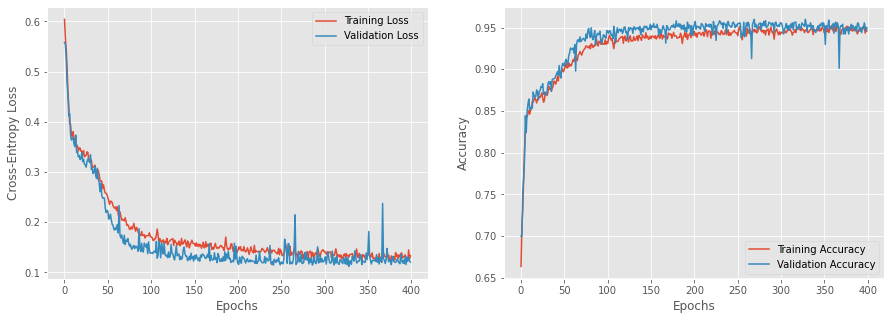
\includegraphics[width=0.9\textwidth]{graphsage_sum_plots.png}
		\caption{Sum-Pooling Aggregation Loss- and Accuracy Plots}
        \label{fig:sum_aggregation}
  \end{figure}

  \noindent The plots show that sum-pooling trains very well. The training 
  accuracy is 94.33\% and validation accuracy is 94.2\% after the model
  finished training. The results for the test graph are shown in table
  \ref{table:sum_results_test}.

  \begin{table}[h]
    \centering
    \begin{tabular}{|l|c|c|}
      \hline
      \diagbox{\textbf{Label}}{\textbf{Predicted}} & \textbf{Neutral or
      Dissatisfied} & \textbf{Satisfied}\\
      \hline
      \textbf{Neutral or Dissatisfied} & 3'218  & 138 \\\hline 
      \textbf{Satisfied} & 212 & 2'432 \\\hline\hline
      \textbf{Accuracy} & 94.17\% & \\
      \hline
    \end{tabular}
    \caption{Test Confusion Matrix Sum-Pooling}
    \label{table:sum_results_test}
  \end{table}

  \paragraph{Max-Pooling Aggregation}  \mbox{}\\ 
  The last aggregation method is max-pooling which yielded similar results as
  sum-pooling. The training- and validation loss as well as the accuracies are 
  shown in figure \ref{fig:max_aggregation}. 

  \begin{figure}[h]
		\centering
		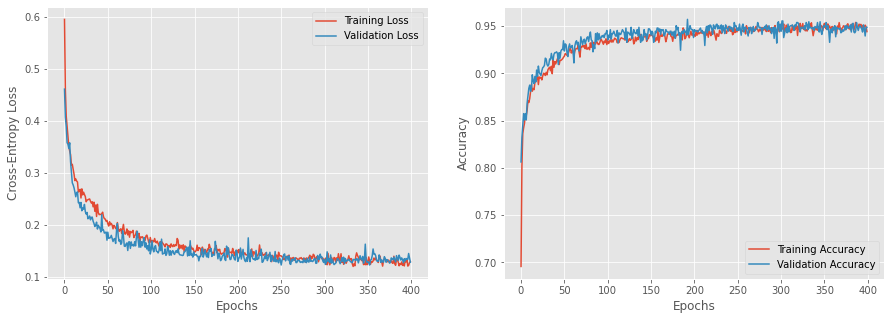
\includegraphics[width=0.9\textwidth]{graphsage_max_plots.png}
		\caption{Max-Pooling Aggregation Loss- and Accuracy Plots}
        \label{fig:max_aggregation}
  \end{figure}

  \noindent The training model resulted with a validation accuracy
  of 93.96\% and training accuracy of 93.84\%. The results for the test graph
  are shown in table \ref{table:max_results_test}.

  \begin{table}[h]
    \centering
    \begin{tabular}{|l|c|c|}
      \hline
      \diagbox{\textbf{Label}}{\textbf{Predicted}} & \textbf{Neutral or
      Dissatisfied} & \textbf{Satisfied}\\
      \hline
      \textbf{Neutral or Dissatisfied} & 3'180  & 176 \\\hline 
      \textbf{Satisfied} & 196 & 2'448 \\\hline\hline
      \textbf{Accuracy} & 93.8\% & \\
      \hline
    \end{tabular}
    \caption{Test Confusion Matrix Max-Pooling}
    \label{table:max_results_test}
  \end{table}

  \subsection{GraphSage Robustness Simulation}
  
  The loss- and accuracy plots reveal mostly a relatively good model fit. LSTM
  aggregation however shows a moderate over-fit and is indicative of a more 
  general issue shown to be true for all aggregation strategies. Simulations
  revealed, that for the same graph the trained model would either over-fit,
  fit perfectly or have a training pattern in which the validation loss was
  smaller than the training loss. An analysis revealed, that the culprit for
  this behavior was the dropout rate of 2\% as well as the random assignment of
  graph nodes into training- and validation data. If the dropout rate was set
  to 0, the model always tended to over-fit, where the training accuracy would
  approach 100\% and the validation accuracy would stagnate around 93-94\%.
  Unfortunately, when applying this model to an unseen test graph, the accuracy
  results were somewhat lower at 91-92\%. For this reason, a dropout rate at
  2\% was set to avoid this over-fitting problem which in turn yielded better
  test results. This has the consequence, that it is more difficult for the
  model to make predictions for the training data compared to the validation
  data which uses no dropout rate. This obstacle however has the downside, that
  it makes the model sensitive to the node assignments during the random
  train- and validation split. Some nodes are more difficult to learn depending
  on their features and neighbors. This means, that if the training set
  includes more difficult nodes on average than the validation set in
  conjunction with the dropout rate as an additional obstacle for the training
  set, the validation loss becomes lower than the training loss. The same is
  true in reverse, which leads to an over-fit. Lastly, the if the nodes in both
  the training- and validation set are on average of similar difficulty a good
  model fit is achieved as shown in the loss- and accuracy plots. \\

  \noindent Nevertheless, the training- and validation results shown are 
  representative for the model in general. In order to show this, a simulation 
  was run using a training- and validation graph consisting of 6'000 nodes and 
  a test graph also consisting of 6'000 nodes. For the simulation, max-pooling 
  aggregation was selected using the same model specifications as previously. 
  The model was trained during 100 experiments, where for every experiment a 
  new random training- and validation split node assignment was performed. The
  trained model was then applied to the test graph where the loss- and accuracy
  was measured. The average results of the 100 experiments are shown in table
  \ref{table:simulation_results} and figure \ref{fig:simulation_results}. 

  \begin{table}[h]
    \centering
      \begin{tabular}{|l||c|c|c|}
      \hline
      \textbf{Metric} & \textbf{Training Set} & \textbf{Validation Set} & 
      \textbf{Test Set}\\
      \hline\hline
      Average Accuracy & 94.37\% & 94.23\% & 93.21\% \\\hline 
      Average Cross-Entropy Loss & 0.3684 & 0.3693 & 0.3792 \\
      \hline
      \end{tabular}
    \caption{Average Simulation Results}
    \label{table:simulation_results}
  \end{table}

  \begin{figure}[h]
		\centering
		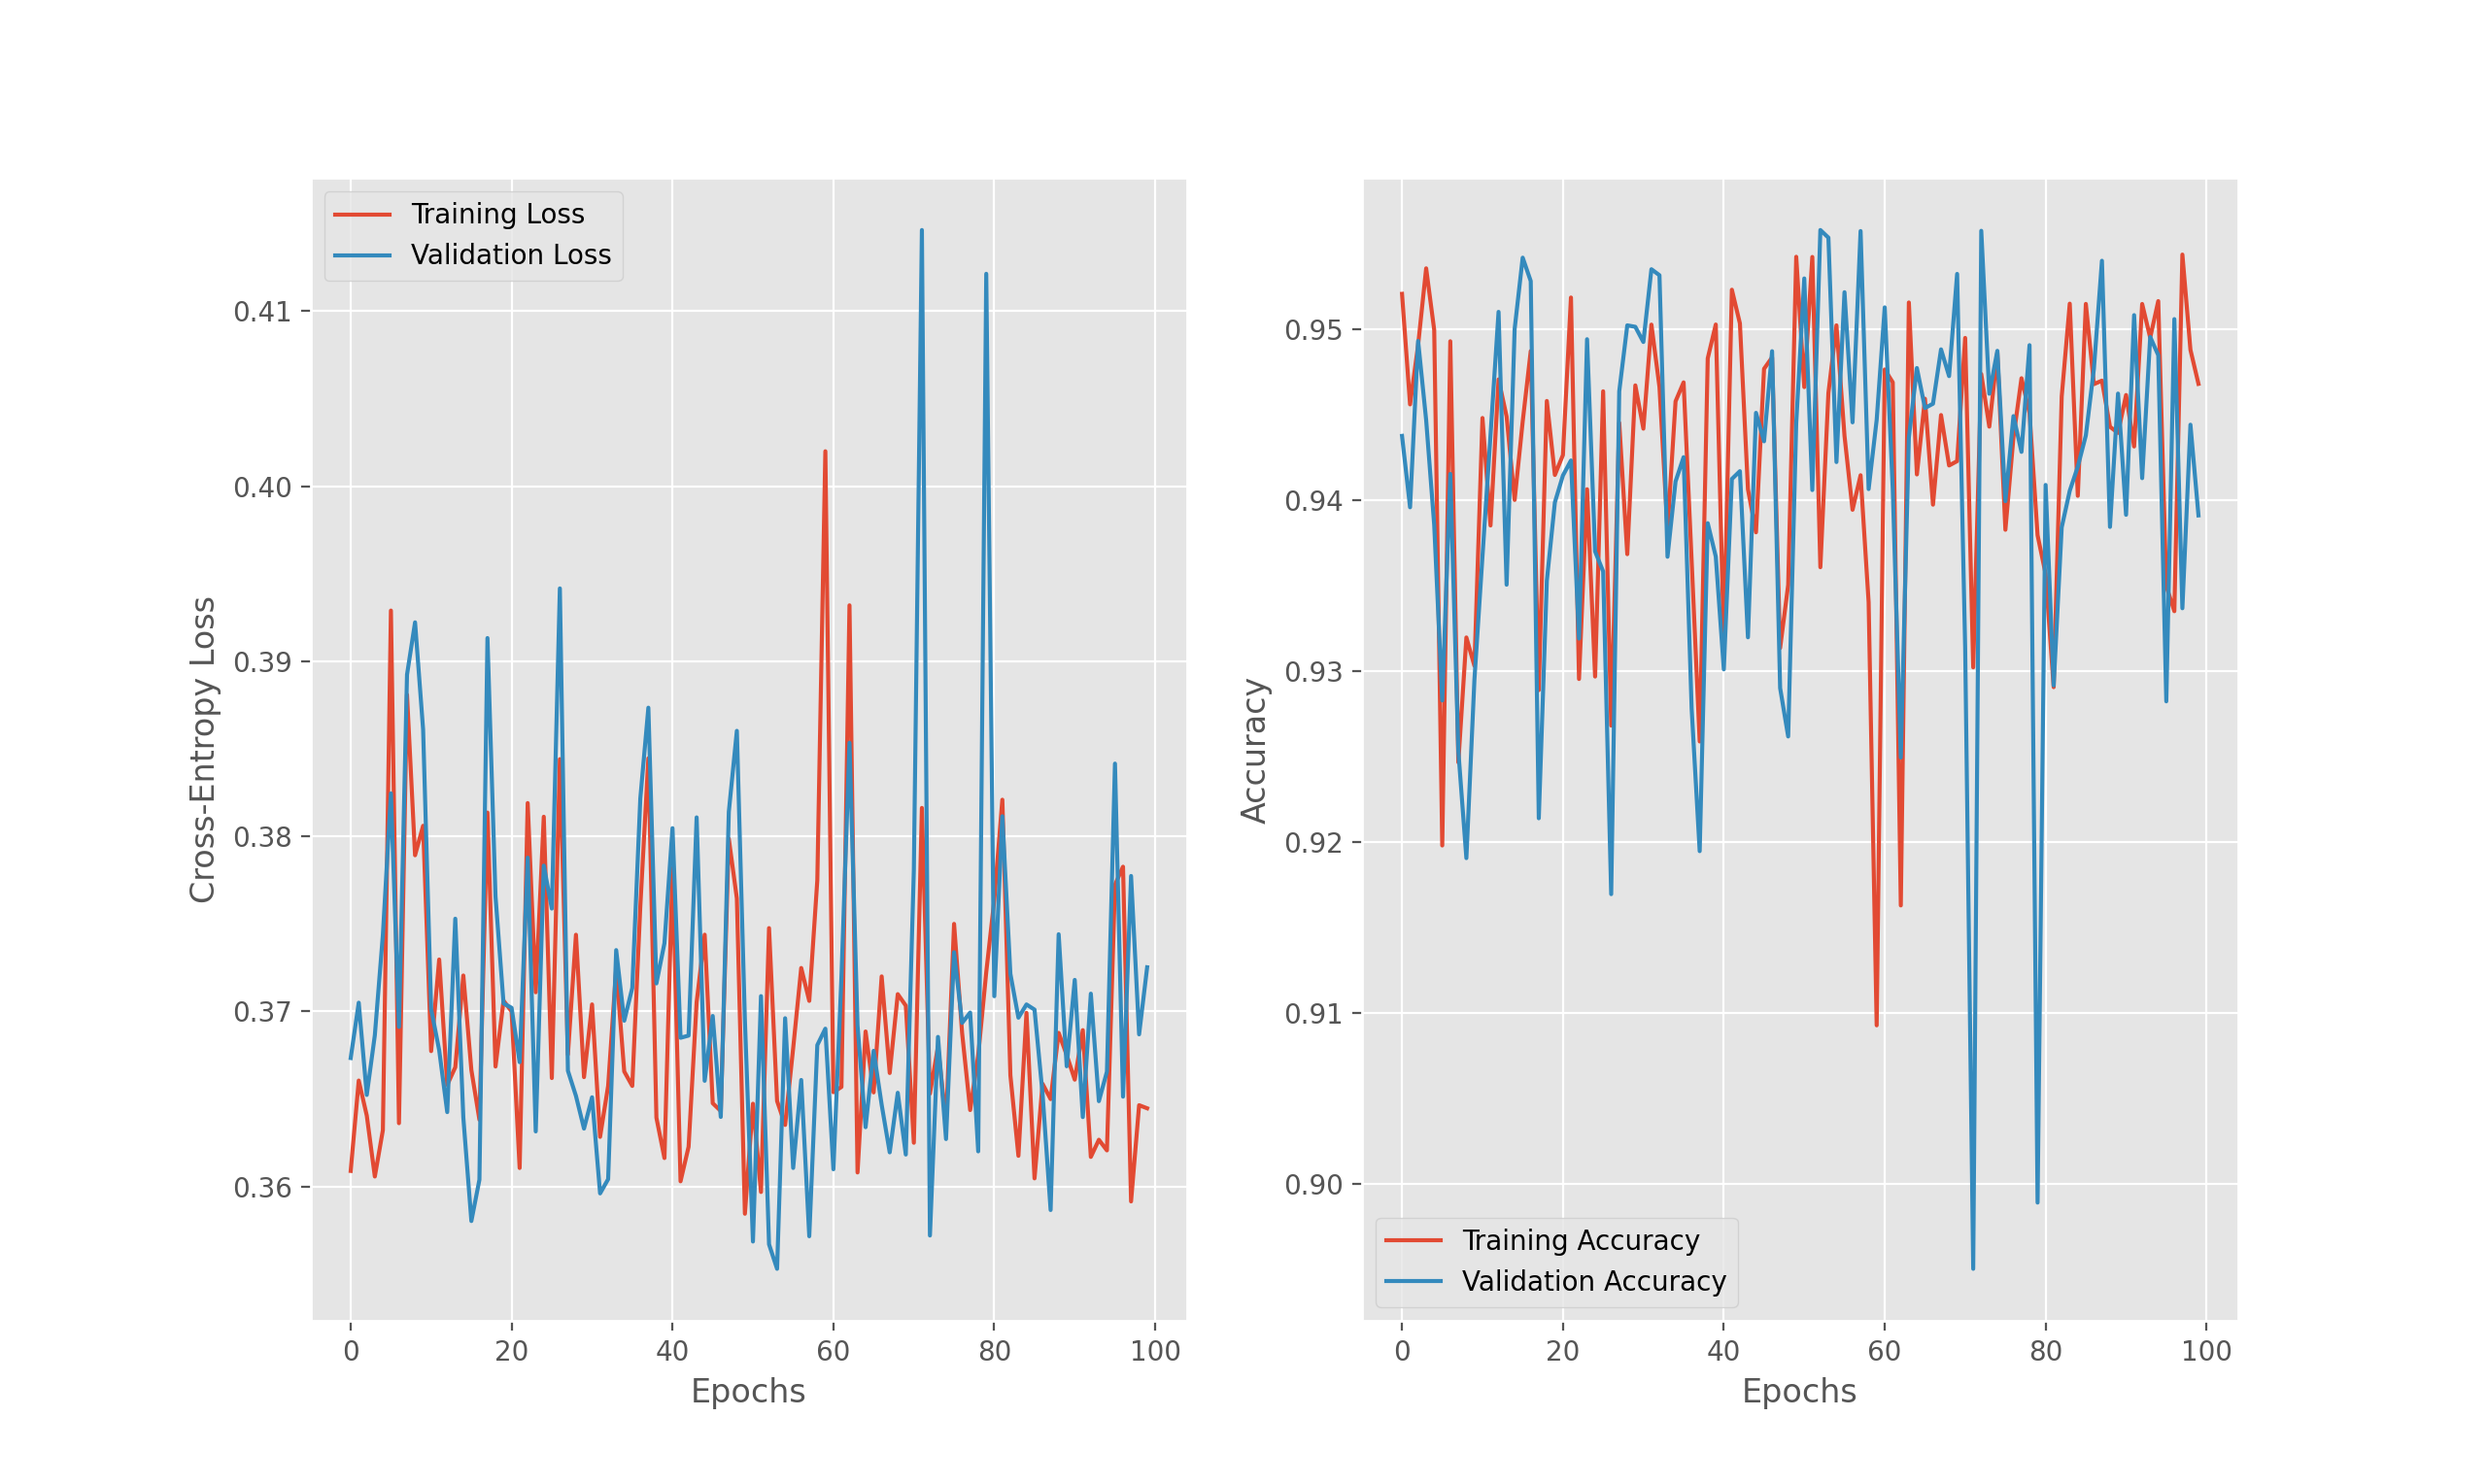
\includegraphics[width=0.9\textwidth]{max_100_sim.png}
		\caption{Simulation Results Max-Pooling}
        \label{fig:simulation_results}
  \end{figure}

  \noindent Max-pooling was selected as this corresponds to the recommended
  aggregation strategy \citep[p. 9]{hamilton2017inductive}. For the remaining
  aggregation strategies, only 10 experiments were run due to time
  considerations as 100 experiments require approximately 15 hours to complete.
  The results using only 10 experiments yielded similar results, with test
  accuracies ranging predominantly from 93-94\%. 

  \section{Result Comparison}
  \label{section:result_comp}

  The results shown for the three models Node2Vec, GCN and GraphSage are
  compared to the results using "standard" machine learning methods. This is
  done to assess to what extent, synthetic graph generation is a useful
  approach for machine learning. This comparison is an important ingredient for
  answering the research question. For the comparison, the methods logistic
  regression \citep{cramer2002origins}, naive bayes \citep{zhang2004bayes},
  support vector machines (SVM) \citep{platt1999probabilistic,chang2011libsvm},
  Random Forest Classifier \citep{breiman2001random}, AdaBoost Classifier
  \citep{freund1997decision,hastie2009multi} and an Artificial Neural Network
  \citep{mcculloch1943logical} are used. These methods only consider the
  feature data and do not consider any network connections. These methods are
  therefore simpler and do not require a graph to be generated. A comparison of
  the different results is shown in table \ref{table:result_comparison}.

  \begin{table}[h]
    \centering
    \scalebox{0.75}{
      \begin{tabular}{|l||c|c|c|}
      \hline
      \textbf{Method} & \textbf{Training Accuracy} & \textbf{Validation
      Accuracy} & \textbf{Test Accuracy}\\
      \hline\hline
      Logistic Regression & 88.16\% & 87.08\% & 86.43\% \\\hline 
      Naive Bayes & 87.46\% & 85.83\% & 85.6\% \\\hline
      AdaBoost & 93.54\% & 93.08\% & 92.45\% \\\hline
      Random Forest & 100\% & 95.08\% & 94.38\% \\\hline
      SVM & 94.42\% & 93.5\% & 92.45\% \\\hline
      ANN & 96.47\% & 94.67\% & 93.32\%\\\hline
      Node2Vec & 77.61\% & 76.58\% & -\\\hline
      GCN & 83.73\% & 82.85\% & -\\\hline
      GraphSage (Mean Aggregation) & 94.98\% & 94.59\% & 93.38\% \\\hline
      GraphSage (LSTM Aggregation) & 94.44\% & 94.09\% & 93.47\% \\\hline
      GraphSage (Sum-Pooling) & 94.33\% & 94.2\% & 94.17\% \\\hline
      GraphSage (Max-Pooling) & 93.96\% & 93.84\% & 93.8\% \\
      \hline
      \end{tabular}}
    \caption{Result Comparison}
    \label{table:result_comparison}
  \end{table}

  \noindent Table \ref{table:result_comparison} shows, that GCN and Node2Vec
  are not competitive when using MAG generated graphs. GraphSage is however a 
  serious competitor and appears to be the second best method overall. The
  Random Forest classifier is consistently the best method regardless of the
  training- and validation data as well as the test data used. The GraphSage
  models are consistently shown to be the second best method. The ANN model
  performs similarly well in terms of achieving a similar test accuracy.
  Similar as with the GNNs, it is important to evaluate the model fit to draw a
  more definitive conclusion which is shown in figure \ref{fig:ANN_fit}.

  \begin{figure}[h]
		\centering
		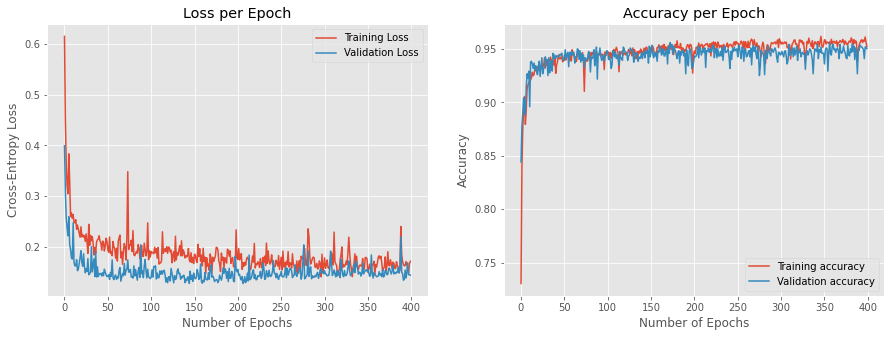
\includegraphics[width=0.9\textwidth]{ANN_Plot.png}
		\caption{ANN Model Fit}
        \label{fig:ANN_fit}
  \end{figure}

  \noindent Figure \ref{fig:ANN_fit} shows, that the ANN model has a relatively
  strong over-fit compared to the GNN models. This observation is consistent
  for every ANN model trained. In addition, different number of hidden layers, 
  hidden layer sizes and dropout rates were tested, which all resulted in a 
  clear over-fit or bad training behavior. For that reason, the ANN is deemed
  to be inferior to the GNN, even if the test accuracies are very similar. \\

  \noindent AdaBoost and SVM also are shown to provide very good results,
  however yield slightly lower test accuracies compared to the previous
  methods. Lastly, naive bayes and logistic regression clearly yield inferior
  results. 
